
%\input{commands}

\newcommand{\mdash}{---}
\newcommand{\q}[1]{``#1''}
\newcommand{\br}{

}

\newcommand{\raggedRightTitle}[1]{\br{}\begin{flushleft}\textbf{#1}\end{flushleft}}

%\newcommand{\visavis}{vis-\`a-vis}


%\input{ngml/ngml-setup-commands}
%\input{ngml/ngml-sdi-commands}
%\input{ngml/ngml-deco-commands}

%\AtEndDocument{\immediate\write18{cd /home/nlevisrael/gits/ntxh/wip-sebi/ar/code/cpp/qmake-console/projects/gtagml/ngml-sdi-console; ./run-with-args.sh /home/nlevisrael/gits/ntxh/wip-sebi/gtagml/ctg/gen/ctg/ctg.gt.tex /home/nlevisrael/gits/ntxh/wip-sebi/gtagml/ctg/gen/ctg/ctg.gt.sdi.ntxh /home/nlevisrael/gits/ntxh/wip-sebi/gtagml/ctg/gen/ctg/ctg.gt.sdi-prelatex.ntxh; cd -;}}



% pmml  arff  openannotation

\usepackage[T1]{fontenc}
\usepackage{tgtermes}

\usepackage[hang,flushmargin]{footmisc}

\usepackage{titlesec}

\titlespacing*{\section}
{0pt}{4ex plus 1ex minus .5ex}{.1ex plus .2ex}

%\usepackage{titlesec}

\titleformat{\section}
  {\normalfont\Large\bfseries}   % The style of the section title
  {}                             % a prefix
  {0pt}                          % How much space exists between the prefix and the title
  {} 


%\usepackage{mathptmx}

\usepackage{eso-pic}

\AddToShipoutPictureBG{%

\colorlet{redbl}{red!40!magenta}
\colorlet{yelbl}{yellow!60!magenta}

\colorlet{redblg}{redbl!30!black}

\ifnum\value{page}>66{
\AtTextLowerLeft{\raisebox{-21pt}{\hspace{-15pt}\fontfamily{qtm}\fontsize{10}{11}\fontseries{b}\selectfont{}{\colorbox{yelbl!7}{\textcolor{redblg!70}{PLEASE SEE OUR SOFTWARE DEMO VIDEOS: \href{http://www.lingtechsys.com/videos/qmt-composite.mkv}{GIS},
\href{http://www.lingtechsys.com/videos/dhax-composite.mkv}{360\textdegree{} photography}, and \href{http://www.lingtechsys.com/videos/xcsd-composite.mkv}{image processing}.}}}}}
}\fi
}


%\setlength\parindent{0pt}

\AddToShipoutPictureBG{%

\ifnum\value{page}>1{
\AtTextUpperLeft{
\makebox[23.1cm][r]{
\raisebox{-.6cm}{%
{\transparent{0.3}{
\includegraphics[width=0.19\textwidth]{e-logo.png}}	}} } }
}\fi
}

\AddToShipoutPicture{%
{
 {\color{blGreen!70!red}\transparent{0.9}{\put(0,0){\rule{3pt}{\paperheight}}}}%
 {\color{darkRed!70!purple}\transparent{1}\put(3,0){{\rule{4pt}{\paperheight}}}}
% {\color{logoPeach!80!cyan}\transparent{0.5}{\put(0,700){\rule{1cm}{.6cm}}}}%
% {\color{darkRed!60!cyan}\transparent{0.7}\put(0,706){{\rule{1cm}{.6cm}}}}
% \put(18,726){\thepage}
% \transparent{0.8}
}
}

%\AddToShipoutPicture{%
%\ifnum\value{page}=1
%\put(247.5,988){%
%	\transparent{0.7}{
%		\includegraphics[width=0.4\textwidth]{logo.png}}}
%\fi
%}	


\AddToShipoutPictureBG{%
\ifnum\value{page}=14

\put(7,678){
	\transparent{1}{
		\includegraphics[angle=0.5,origin=c,width=0.4\textwidth]{pm/1a.jpg}}}


\put(241,698){
	\transparent{1}{
		\includegraphics[angle=0,origin=c,width=0.31\textwidth,
trim=0 14mm 0 10mm, clip]{pm/7a.png}}}


\put(6,492){
	\transparent{1}{
		\includegraphics[angle=-0.5,origin=c,width=0.4\textwidth]{pm/5a.png}}}


\put(452,712){
	\transparent{1}{
		\includegraphics[angle=-1,origin=c,width=0.3\textwidth]{pm/2a.png}}}



\put(442,681){
	\transparent{1}{
		\includegraphics[angle=0,origin=c,width=0.18\textwidth]{pm/8a.png}}}


%\put(412,680){
%	\transparent{1}{
%		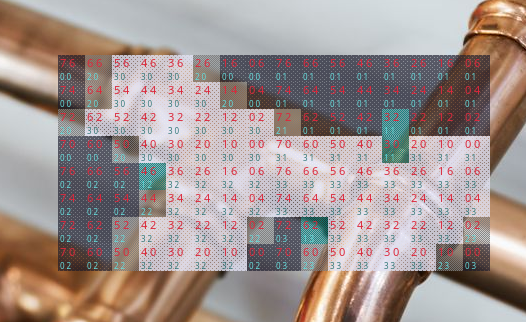
\includegraphics[angle=2.5,origin=c,width=0.2\textwidth]{pm/8.png}}}


\put(402,487){
	\transparent{1}{
		\includegraphics[angle=-1,origin=c,width=0.45\textwidth]{pm/3a.jpg}}}

\fi
}	




%\pagestyle{empty} % no page number
%\parskip 7.2pt    % space between paragraphs
%\parindent 12pt   % indent for new paragraph
%\textwidth 4.5in  % width of text
%\columnsep 0.8in  % separation between columns

%\setlength{\footskip}{-3pt}

%\usepackage[paperheight=15in,paperwidth=8.5in]{geometry}
%\geometry{left=.65in,top=.65in,right=.45in,bottom=1.25in} %margins

%\renewcommand{\thepage}{\raisebox{2pt}{\arabic{page}}}

\renewcommand{\footnoterule}{%
	\kern -3pt
	\hrule width .92\textwidth height .5pt
	\kern 10pt
}


\usepackage[hyphens]{url}
\newcommand{\biburl}[1]{ {\fontfamily{gar}\selectfont{\textcolor[rgb]{.2,.6,0}%
{\scriptsize {\url{#1}}}}}}

\newcommand{\bhref}[1]{\href{#1}{#1}}



%\linespread{1.3}

\newcommand{\sectsp}{\vspace{12pt}}

\usepackage{graphicx}
\usepackage{color,framed}

\usepackage{textcomp}

\usepackage{float}

\usepackage{mdframed}


\usepackage{setspace}

\usepackage{xcolor}

\usepackage[hyphenbreaks]{breakurl}
\usepackage[hyphens]{url}

%\usepackage{hyperref}

\colorlet{blCyan}{cyan!50!blue}

\definecolor{darkRed}{rgb}{.2,.0,.1}


\definecolor{blGreen}{rgb}{.2,.7,.3}

\definecolor{darkBlGreen}{rgb}{.1,.3,.2}

\definecolor{oldBlColor}{rgb}{.2,.7,.3}

\definecolor{blColor}{rgb}{.1,.3,.2}

\definecolor{elColor}{rgb}{.2,.1,0}
\definecolor{flColor}{rgb}{0.7,0.3,0.3}

\definecolor{logoOrange}{RGB}{108, 18, 30}
\definecolor{logoGreen}{RGB}{85, 153, 89}
\definecolor{logoPurple}{RGB}{200, 208, 30}

\definecolor{logoBlue}{RGB}{4, 2, 25}
\definecolor{logoPeach}{RGB}{255, 159, 102}
\definecolor{logoCyan}{RGB}{66, 206, 244}
\definecolor{logoRed}{rgb}{.3,0,0}

\newcommand{\colorq}[1]{{\color{logoOrange!70!black}{\q{\small\textbf{#1}}}}}

\let\qq\q

\definecolor{inOne}{rgb}{0.122, 0.435, 0.698}% Rule colour
\definecolor{inTwo}{rgb}{0.122, 0.698, 0.435}% Rule colour

\definecolor{outOne}{rgb}{0.435, 0.698, 0.122}% Rule colour
\definecolor{outTwo}{rgb}{0.698, 0.435, 0.122}% Rule colour

\colorlet{linkcolor}{flColor!60!red}




\usepackage[many]{tcolorbox}% http://ctan.org/pkg/tcolorbox

\usepackage{transparent}

\newlength{\bsep}
\setlength{\bsep}{-1pt}
\let\xbibitem\bibitem
\renewcommand{\bibitem}[2]{\vspace{\bsep}\xbibitem{#1}{#2}}

\newenvironment{cframed}{\begin{mdframed}[linecolor=logoPeach,linewidth=0.4mm]}{\end{mdframed}}

\newenvironment{ccframed}{\begin{mdframed}[backgroundcolor=logoGreen!5,linecolor=logoCyan!50!black,linewidth=0.4mm]}{\end{mdframed}}

\usepackage{aurical}
\usepackage[T1]{fontenc}

\usepackage{relsize}

\newcommand{\bref}[1]{\hspace*{1pt}\textbf{\ref{#1}}}

\newcommand{\dashsep}{--\hspace*{5pt}}

\newcommand{\pseudoIndent}{

\vspace{2pt}\hspace*{6pt}}

\usepackage{titlesec}

\titlespacing*{\subsection}
{0pt}{5ex plus 1ex minus .2ex}{0.5ex plus .2ex}


%\titlespacing*{\section}
%{0pt}{3.5ex plus 1ex minus .2ex}{1ex plus .2ex}

%
\newcommand{\deconum}[1]{{\protect\raisebox{-1pt}{{\LARGE #1}}}}

\newcommand{\visavis}{vis-\`a-vis}

\newcommand{\VersatileUX}{{\color{red!85!black}{\Fontauri Versatile}}%
{{\fontfamily{qhv}\selectfont\smaller UX}}}

\newcommand{\NDPCloud}{{\color{red!15!black}%
{\fontfamily{qhv}\selectfont {\smaller NDP C{\smaller LOUD}}}}}

\newcommand{\MThreeK}{{\color{blGreen!45!black}%
{\fontfamily{qhv}\fontsize{10}{8}\selectfont {M3K}}}}


\newcommand{\lfNDPCloud}{{\color{red!15!black}%
{\fontfamily{qhv}\selectfont N{\smaller DP C{\smaller LOUD}}}}}

\newcommand{\textds}[1]{{\fontfamily{lmdh}\selectfont{%
\raisebox{-1pt}{#1}}}}

\newcommand{\dsC}{{\textds{ds}{\fontfamily{qhv}\selectfont \raisebox{-1pt}
{\color{red!15!black}{C}}}}}

\definecolor{tcolor}{RGB}{24,52,61}

\newcommand{\CCpp}{\resizebox{!}{7pt}{\AcronymText{C}}/\Cpp{}}
\newcommand{\NoSQL}{\resizebox{!}{6.5pt}{\AcronymText{NoSQL}}}
\newcommand{\SQL}{\resizebox{!}{7pt}{\AcronymText{SQL}}}

\newcommand{\NCBI}{\resizebox{!}{7pt}{\AcronymText{NCBI}}}
\newcommand{\BioNetGen}{\resizebox{!}{7pt}{\AcronymText{BioNetGen}}}
\newcommand{\BNGL}{\resizebox{!}{7pt}{\AcronymText{BNGL}}}

\newcommand{\GML}{\resizebox{!}{7pt}{\AcronymText{GML}}}

\newcommand{\GIS}{\resizebox{!}{6.5pt}{\AcronymText{GIS}}}
\newcommand{\ACRIS}{\resizebox{!}{6.5pt}{\AcronymText{ACRIS}}}
\newcommand{\HPD}{\resizebox{!}{6.5pt}{\AcronymText{HPD}}}


\newcommand{\HTXN}{\resizebox{!}{7pt}{\AcronymText{HTXN}}}

\newcommand{\TDM}{\resizebox{!}{7pt}{\AcronymText{TDM}}}

\newcommand{\lHTXN}{\resizebox{!}{7.5pt}{\AcronymText{H}}%
\resizebox{!}{6.5pt}{\AcronymText{TXN}}}

\newcommand{\lsHTXN}{\resizebox{!}{9.5pt}{\AcronymText{\textcolor{tcolor}{HTXN}}}}

\newcommand{\LAF}{\resizebox{!}{7pt}{\AcronymText{LAF}}}

\newcommand{\UDpipe}{\resizebox{!}{7pt}{\AcronymText{UDpipe}}}

\newcommand{\C}{\resizebox{!}{7pt}{\AcronymText{C}}}

\newcommand{\TME}{\resizebox{!}{7pt}{\AcronymText{TME}}}

\newcommand{\TwoD}{\resizebox{!}{6.5pt}{\AcronymText{2D}}}




\usepackage{mdframed}

\newcommand{\cframedboxpanda}[1]{\begin{mdframed}[linecolor=yellow!70!blue,linewidth=0.4mm]#1\end{mdframed}}





\newcommand{\libSBML}{\resizebox{!}{7pt}{\AcronymText{libSBML}}}


\newcommand{\PVD}{\resizebox{!}{7pt}{\AcronymText{PVD}}}


\newcommand{\SDK}{\resizebox{!}{7pt}{\AcronymText{SDK}}}
\newcommand{\NLP}{\resizebox{!}{7pt}{\AcronymText{NLP}}}


\newcommand{\PDF}{\resizebox{!}{6.5pt}{\AcronymText{PDF}}}
\newcommand{\TEI}{\resizebox{!}{7.5pt}{\AcronymText{TE{\hspace*{.5pt}I}}}}
\newcommand{\SSML}{\resizebox{!}{7.5pt}{\AcronymText{SSML}}}
\newcommand{\ToBI}{\resizebox{!}{7.5pt}{\AcronymText{ToBI}}}

\newcommand{\MMBioS}{\resizebox{!}{6.5pt}{\AcronymText{MMBioS}}}

\newcommand{\VTK}{\resizebox{!}{6.5pt}{\AcronymText{VTK}}}


\newcommand{\AXF}{\resizebox{!}{7pt}{\AcronymText{AXF}}}

\newcommand{\HyperGraphDB}{\resizebox{!}{7pt}{\AcronymText{HyperGraphDB}}}


\newcommand{\lAXF}{\resizebox{!}{7.5pt}{\AcronymText{A}}%
\resizebox{!}{6.5pt}{\AcronymText{XF}}}


\newcommand{\lsAXF}{\resizebox{!}{8.5pt}{\AcronymText{AXF}}}

\newcommand{\AXFD}{\resizebox{!}{7pt}{\AcronymText{AXFD}}}

\newcommand{\lAXFD}{\resizebox{!}{7.5pt}{\AcronymText{A}}%
\resizebox{!}{6.5pt}{\AcronymText{XFD}}}


\newcommand{\IJST}{\resizebox{!}{7pt}{\AcronymText{IJST}}}

\newcommand{\BioC}{\resizebox{!}{7pt}{\AcronymText{BioC}}}

\newcommand{\CoNLL}{\resizebox{!}{7pt}{\AcronymText{CoNLL}}}
\newcommand{\CoNLLU}{\resizebox{!}{7pt}{\AcronymText{CoNLL-U}}}


\newcommand{\ePub}{\resizebox{!}{7pt}{\AcronymText{ePub}}}

%\lsLPF

\definecolor{atcColor}{RGB}{96, 17, 12}
%\textcolor{tcolor}{

\newcommand{\ATextCClr}[1]{\textcolor{atcColor}{\textbf{#1}}}

\newcommand{\ATexttclr}[1]{\textcolor{tcolor}{\textbf{#1}}}
\newcommand{\THQL}{\resizebox{!}{6.5pt}{\ATexttclr{THQL}}}


\newcommand{\ATextbk}[1]{\textcolor{black!50!cyan}{\textbf{#1}}}


%\newcommand{\lDHOS}{\resizebox{!}{7pt}{\ATexttclr{D}}%
%resizebox{!}{6.5pt}{\ATexttclr{HOS}}}

\newcommand{\PGVM}{\resizebox{!}{6.5pt}{\ATexttclr{PGVM}}}
\newcommand{\lPGVM}{\resizebox{!}{7pt}{\ATexttclr{PGVM}}}

\newcommand{\DHOS}{\resizebox{!}{6.5pt}{\ATexttclr{DHOS}}}
\newcommand{\lDHOS}{\resizebox{!}{7.5pt}{\ATexttclr{D}}\resizebox{!}{6.5pt}{\ATexttclr{HOS}}}
\newcommand{\sDHOS}{\resizebox{!}{6.5pt}{\ATexttclr{DHOS}}}

\newcommand{\sQt}{\resizebox{!}{6.5pt}{\ATexttclr{Qt}}}

\newcommand{\sPhVM}{\resizebox{!}{6.5pt}{\ATexttclr{P\hspace{.5pt}\textit{h}\hspace*{-.5pt}VM}}}


\newcommand{\PhVM}{\resizebox{!}{6.5pt}{\ATexttclr{P\hspace{.5pt}\textit{h}\hspace*{-.5pt}VM}}}
\newcommand{\lPhVM}{\resizebox{!}{7.5pt}{\ATexttclr{P}}\resizebox{!}{6.5pt}{\ATexttclr{\hspace{1pt}\textit{h}\hspace*{-.5pt}VM}}}


\newcommand{\MOC}{\resizebox{!}{7pt}{\AcronymText{MOC}}}
\newcommand{\SPARQL}{\resizebox{!}{7pt}{\AcronymText{SPARQL}}}
\newcommand{\GraphQL}{\resizebox{!}{7pt}{\AcronymText{GraphQL}}}

%{}, \QML{}, \GraphQL

\newcommand{\CCi}{\resizebox{!}{6.5pt}{\ATexttclr{CCi}}}
\newcommand{\XCSD}{\resizebox{!}{6.5pt}{\ATexttclr{XCSD}}}

\newcommand{\lXCSD}{\resizebox{!}{7pt}{\ATexttclr{XCSD}}}
\newcommand{\lCCi}{\resizebox{!}{7pt}{\ATexttclr{CCi}}}

%\newcommand{\ConceptsDB}{\resizebox{!}{6.5pt}{\ATexttclr{ConceptsDB}}}
%\newcommand{\lConceptsDB}{\resizebox{!}{7pt}{\ATexttclr{C}}\resizebox{!}{6.5pt}%{\ATexttclr{onceptsDB}}}


\newcommand{\GIT}{\resizebox{!}{7pt}{\AcronymText{GIT}}}

\newcommand{\LPF}{\resizebox{!}{7pt}{\AcronymText{LPF}}}
\newcommand{\lLPF}{\resizebox{!}{8.5pt}{\AcronymText{LPF}}}
\newcommand{\lsLPF}{\resizebox{!}{9.5pt}{\AcronymText{LPF}}}

\makeatletter

\newcommand*\getX[1]{\expandafter\getX@i#1\@nil}

\newcommand*\getY[1]{\expandafter\getY@i#1\@nil}
\def\getX@i#1,#2\@nil{#1}
\def\getY@i#1,#2\@nil{#2}
\makeatother
	
\newcommand{\rectann}[9]{%
\path [draw=#1,draw opacity=#2,line width=#3, fill=#4, fill opacity = #5, even odd rule] %
(#6) rectangle(\getX{#6}+#7,\getY{#6}+#8)
({\getX{#6}+((#7-(#7*#9))/2)},{\getY{#6}+((#8-(#8*#9))/2)}) rectangle %
({\getX{#6}+((#7-(#7*#9))/2)+#7*#9},{\getY{#6}+((#8-(#8*#9))/2)+#8*#9});}


\definecolor{pfcolor}{RGB}{94, 54, 73}

\newcommand{\EPF}{\resizebox{!}{7pt}{\AcronymText{ETS{\color{pfcolor}pf}}}}
\newcommand{\lEPF}{\resizebox{!}{8.5pt}{\AcronymText{ETS{\color{pfcolor}pf}}}}
\newcommand{\lsEPF}{\resizebox{!}{9.5pt}{\AcronymText{ETS{\color{pfcolor}pf}}}}

\newcommand{\RGB}{\resizebox{!}{6.5pt}{\AcronymText{RGB}}}


\newcommand{\GRE}{\resizebox{!}{7pt}{\AcronymText{GRE}}}
\newcommand{\CAS}{\resizebox{!}{7pt}{\AcronymText{CAS}}}

\newcommand{\lMOSAIC}{%
\resizebox{!}{8pt}{\AcronymText{M}}%
\resizebox{!}{6.5pt}{\AcronymText{OSAIC}}}

\newcommand{\XML}{\resizebox{!}{7pt}{\AcronymText{XML}}}
\newcommand{\RDF}{\resizebox{!}{7pt}{\AcronymText{RDF}}}
\newcommand{\DOM}{\resizebox{!}{7pt}{\AcronymText{DOM}}}


\newcommand{\CWL}{\resizebox{!}{7pt}{\AcronymText{CWL}}}




\newcommand{\Covid}{\resizebox{!}{7pt}{\AcronymText{Covid-19}}}

\newcommand{\CLang}{\resizebox{!}{7pt}{\AcronymText{C}}}

\newcommand{\HNaN}{\resizebox{!}{7pt}{\AcronymText{HN%
\textsc{a}N}}}

\newcommand{\JSON}{\resizebox{!}{7pt}{\AcronymText{JSON}}}

\newcommand{\MeshLab}{\resizebox{!}{7pt}{\AcronymText{MeshLab}}}
%\newcommand{\IQmol}{\resizebox{!}{7pt}{\AcronymText{IQmol}}}

\newcommand{\SGML}{\resizebox{!}{7pt}{\AcronymText{SGML}}}

\newcommand{\ASCII}{\resizebox{!}{7pt}{\AcronymText{ASCII}}}



\newcommand{\JATS}{\resizebox{!}{7pt}{\AcronymText{JATS}}}


\newcommand{\SDI}{\resizebox{!}{7pt}{\AcronymText{SDI}}}
\newcommand{\SDIV}{\resizebox{!}{7pt}{\AcronymText{SDIV}}}

\newcommand{\VXL}{\resizebox{!}{7pt}{\AcronymText{VXL}}}
\newcommand{\IQmol}{\resizebox{!}{7pt}{\AcronymText{IQmol}}}




\newcommand{\VM}{\resizebox{!}{7pt}{\AcronymText{VM}}}
\newcommand{\sVM}{\resizebox{!}{6.5pt}{\AcronymText{VM}}}


\newcommand{\IDE}{\resizebox{!}{7pt}{\AcronymText{IDE}}}


\newcommand{\OS}{\resizebox{!}{7pt}{\AcronymText{OS}}}

\newcommand{\FAIR}{\resizebox{!}{7pt}{\AcronymText{FAIR}}}
\newcommand{\FAIRsharing}{\resizebox{!}{7pt}{\AcronymText{FAIR}}\hspace*{1pt}\resizebox{!}{8pt}{sharing}}

\newcommand{\Python}{\resizebox{!}{7pt}{\AcronymText{Python}}}
\newcommand{\RPC}{\resizebox{!}{7pt}{\AcronymText{RPC}}}

\newcommand{\Java}{\resizebox{!}{7pt}{\AcronymText{Java}}}

\newcommand{\sBioNetGen}{\resizebox{!}{6.5pt}{\AcronymText{BioNetGen}}}
\newcommand{\sUI}{\resizebox{!}{6.5pt}{\AcronymText{UI}}}
\newcommand{\sAPOLLO}{\resizebox{!}{6.5pt}{\AcronymText{APOLLO}}}
\newcommand{\sSDK}{\resizebox{!}{6.5pt}{\AcronymText{SDK}}}
\newcommand{\sGUI}{\resizebox{!}{6.5pt}{\AcronymText{GUI}}}
\newcommand{\sAPI}{\resizebox{!}{6.5pt}{\AcronymText{API}}}




\newcommand{\QNetworkManager}{\resizebox{!}{7pt}{\AcronymText{QNetworkManager}}}
\newcommand{\QTextDocument}{\resizebox{!}{7pt}{\AcronymText{QTextDocument}}}

\newcommand{\QWebEngineView}{\resizebox{!}{6.5pt}{\AcronymText{QWebEngineView}}}

\newcommand{\HTTP}{\resizebox{!}{6.5pt}{\AcronymText{HTTP}}}


\newcommand{\lAcronymTextNC}[2]{{\fontfamily{fvs}\selectfont {\Large{#1}}{\large{#2}}}}

\newcommand{\AcronymTextNC}[1]{{\fontfamily{fvs}\selectfont {\large #1}}}



\colorlet{orr}{orange!60!red}

\colorlet{orb}{green!60!blue}
\colorlet{orbb}{green!30!blue}



\newcommand{\usstitle}[1]{\vspace{.4em}\raisebox{-1.2em}{{\fontfamily{gar}\fontsize{12}{14}%
\fontseries{sb}\selectfont{{\textcolor{orbb!65!black}{#1}}}}}}}


\newcommand{\sstitle}[1]{\vspace{1.4em}\raisebox{-1.2em}{{\fontfamily{gar}\fontsize{12}{14}%
\fontseries{sb}\selectfont{{\textcolor{orbb!65!black}{#1}}}}}}}

\newcommand{\DaSemio}{{\fontfamily{fvs}\fontsize{9}{14}%
\selectfont{\textbf{\textcolor{orb!75!black}{Da\resizebox{6pt}{!}{S}emio}}}}}}


\newcommand{\lDaSemio}{{\fontfamily{fvs}\fontsize{9}{14}%
\selectfont{\textbf{\textcolor{orb!75!black}{\resizebox{9pt}{!}{D}aSemio}}}}}}


%\newcommand{\DaSemio}{DaSemio}



\newcommand{\textscci}[1]{{\color{orr!35!black}{{%
						\fontfamily{Cabin-TLF}\fontseries{b}\selectfont{\textit{\scriptsize{#1}}}}}}}


\newcommand{\textscc}[1]{{\color{orr!35!black}{{%
						\fontfamily{Cabin-TLF}\fontseries{b}\selectfont{\textsc{\scriptsize{#1}}}}}}}


\newcommand{\textsccserif}[1]{{\color{orr!35!black}{{%
				\scriptsize{\textbf{#1}}}}}}


\newcommand{\iEPF}{\resizebox{!}{7pt}{\textsccserif{%
\textit{ETSpf}}}}

\newcommand{\iSDI}{\resizebox{!}{7pt}{\textsccserif{%
\textit{SDI}}}}

\newcommand{\iHTXN}{\resizebox{!}{7pt}{\textsccserif{%
\textit{HTXN}}}}




\newcommand{\AcronymText}[1]{{\textscc{#1}}}
\newcommand{\iAcronymText}[1]{{\textscci{#1}}}

\newcommand{\AcronymTextser}[1]{{\textsccserif{#1}}}


\newcommand{\mAcronymText}[1]{{\textscc{\normalsize{#1}}}}

\newcommand{\FASTA}{{\resizebox{!}{7pt}{\AcronymText{FASTA}}}}
\newcommand{\SRA}{{\resizebox{!}{7pt}{\AcronymText{SRA}}}}
\newcommand{\DNA}{{\resizebox{!}{7pt}{\AcronymText{DNA}}}}
\newcommand{\MAP}{{\resizebox{!}{7pt}{\AcronymText{MAP}}}}
\newcommand{\EPS}{{\resizebox{!}{7pt}{\AcronymText{EPS}}}}

\newcommand{\CSV}{{\resizebox{!}{6.5pt}{\AcronymText{CSV}}}}

%\newcommand{\PDB}{{\resizebox{!}{7pt}{\AcronymText{PDB}}}}


\newcommand{\APOLLO}{{\resizebox{!}{7pt}{\AcronymText{APOLLO}}}}
\newcommand{\GDC}{{\resizebox{!}{7pt}{\AcronymText{GDC}}}}
\newcommand{\TCIA}{{\resizebox{!}{7pt}{\AcronymText{TCIA}}}}
\newcommand{\CPTAC}{{\resizebox{!}{7pt}{\AcronymText{CPTAC}}}}





\newcommand{\XOCS}{{\resizebox{!}{7pt}{\AcronymText{XOCS}}}}


\newcommand{\cytoLib}{{\resizebox{!}{7pt}{\AcronymText{cytoLib}}}}
\newcommand{\CaPTk}{{\resizebox{!}{7pt}{\AcronymText{CaPTk}}}}
\newcommand{\DCMTK}{{\resizebox{!}{7pt}{\AcronymText{DCMTK}}}}
%\newcommand{\VM}{{\resizebox{!}{7pt}{\AcronymText{VM}}}}
\newcommand{\DSL}{{\resizebox{!}{7pt}{\AcronymText{DSL}}}}
\newcommand{\Paraview}{{\resizebox{!}{7pt}{\AcronymText{ParaView}}}}
\newcommand{\BFP}{{\resizebox{!}{7pt}{\AcronymText{BFP}}}}





\newcommand{\ChemXML}{{\resizebox{!}{7pt}{\AcronymText{ChemXML}}}}

\newcommand{\TeXMECS}{\resizebox{!}{7pt}{\AcronymText{TeXMECS}}}

% pmml  arff  openannotation

\newcommand{\PMML}{\resizebox{!}{7pt}{\AcronymText{PMML}}}
\newcommand{\ARFF}{\resizebox{!}{7pt}{\AcronymText{ARFF}}}
\newcommand{\IeXML}{\resizebox{!}{7pt}{\AcronymText{IeXML}}}


\newcommand{\NGML}{\resizebox{!}{7pt}{\AcronymText{NGML}}}


\newcommand{\WhiteDB}{\resizebox{!}{7pt}{\AcronymText{WhiteDB}}}

\colorlet{drp}{darkRed!70!purple}

%\newcommand{\MOSAIC}{{\color{drp}{\AcronymTextNC{\scriptsize{MOSAIC}}}}}

\newcommand{\MOSAIC}{\resizebox{!}{7pt}{\AcronymText{MOSAIC}}}


\newcommand{\mMOSAIC}{{\color{drp}{\AcronymTextNC{\normalsize{MOSAIC}}}}}

\newcommand{\MOSAICVM}{\mMOSAIC-\mAcronymText{VM}}

\newcommand{\sMOSAICVM}{\resizebox{!}{7pt}{\MOSAICVM}}
\newcommand{\sMOSAIC}{\resizebox{!}{7pt}{\MOSAIC}}

\newcommand{\LDOM}{\resizebox{!}{7pt}{\AcronymText{LDOM}}}
\newcommand{\Cnineteen}{\resizebox{!}{7pt}{\AcronymText{CORD-19}}}

\newcommand{\lCnineteen}{\resizebox{!}{7.5pt}{\AcronymText{CORD-19}}}


\newcommand{\MOL}{\resizebox{!}{7pt}{\AcronymText{MOL}}}

\newcommand{\ACL}{\resizebox{!}{7pt}{\AcronymText{ACL}}}

\newcommand{\LXCR}{\resizebox{!}{7pt}{\AcronymText{LXCR}}}
\newcommand{\lLXCR}{\resizebox{!}{8.5pt}{\AcronymText{LXCR}}}
\newcommand{\lsLXCR}{\resizebox{!}{9.5pt}{\AcronymText{LXCR}}}

%\newcommand{\lMOSAIC}{{\color{drp}{\lAcronymTextNC{M}{OSAIC}}}}
\newcommand{\lfMOSAIC}{\resizebox{!}{9pt}{{\color{drp}{\lAcronymTextNC{M}{OSAIC}}}}}

\newcommand{\Mosaic}{\resizebox{!}{7pt}{\MOSAIC}}
\newcommand{\MosaicPortal}{{\color{drp}{\AcronymTextNC{MOSAIC Portal}}}}

\newcommand{\RnD}{\resizebox{!}{7pt}{\AcronymText{R\&D}}}

\newcommand{\Cpp}{\resizebox{!}{6.5pt}{\AcronymText{C++}}}
\newcommand{\sRPC}{\resizebox{!}{6.5pt}{\AcronymText{RPC}}}



\newcommand{\JavaScript}{\resizebox{!}{6.5pt}{\AcronymText{JavaScript}}}


\newcommand{\Qt}{\resizebox{!}{6.5pt}{\AcronymText{Qt}}}


\newcommand{\DICOM}{\resizebox{!}{6.5pt}{\AcronymText{DICOM}}}
\newcommand{\TIFF}{\resizebox{!}{6.5pt}{\AcronymText{TIFF}}}


\newcommand{\WSI}{\resizebox{!}{7.5pt}{\AcronymText{WSI}}}

\newcommand{\ITK}{\resizebox{!}{6.5pt}{\AcronymText{ITK}}}

\newcommand{\medInria}{\resizebox{!}{7.5pt}{\AcronymText{medInria}}}

\newcommand{\OpenCV}{\resizebox{!}{6.5pt}{\AcronymText{OpenCV}}}
\newcommand{\CvMat}{\resizebox{!}{6.5pt}{\AcronymText{CvMat}}}

\newcommand{\MTA}{\resizebox{!}{6.5pt}{\AcronymText{MTA}}}

\newcommand{\XYZ}{\resizebox{!}{6.5pt}{\AcronymText{XYZ}}}
\newcommand{\ULURP}{\resizebox{!}{6.5pt}{\AcronymText{ULURP}}}

\newcommand{\CEQR}{\resizebox{!}{6.5pt}{\AcronymText{CEQR}}}


\newcommand{\SLD}{\resizebox{!}{6.5pt}{\AcronymText{SLD}}}
\newcommand{\FITS}{\resizebox{!}{6.5pt}{\AcronymText{FITS}}}

\newcommand{\REST}{\resizebox{!}{6.5pt}{\AcronymText{REST}}}

\newcommand{\LLVM}{\resizebox{!}{6.5pt}{\AcronymText{LLVM}}}
\newcommand{\JVM}{\resizebox{!}{6.5pt}{\AcronymText{JVM}}}

\newcommand{\TRI}{\resizebox{!}{6.5pt}{\AcronymText{TRI}}}

\newcommand{\PFAS}{\resizebox{!}{6.5pt}{\AcronymText{PFAS}}}
\newcommand{\EPA}{\resizebox{!}{6.5pt}{\AcronymText{EPA}}}




\newcommand{\lVM}{\resizebox{!}{7pt}{VM}}
\newcommand{\stGUI}{\resizebox{!}{7pt}{GUI}}

\newcommand{\HDFfive}{\resizebox{!}{6.5pt}{\AcronymText{HDF5}}}
\newcommand{\HDFfour}{\resizebox{!}{6.5pt}{\AcronymText{HDF4}}}


\newcommand{\HfiveIM}{\resizebox{!}{6.5pt}{\AcronymText{H5IM}}}


\newcommand{\HDF}{\resizebox{!}{6.5pt}{\AcronymText{HDF}}}
\newcommand{\CDF}{\resizebox{!}{6.5pt}{\AcronymText{CDF}}}
\newcommand{\netCDF}{\resizebox{!}{6.5pt}{\AcronymText{netCDF}}}

\newcommand{\QGIS}{\resizebox{!}{6.5pt}{\AcronymText{QGIS}}}


\newcommand{\QtSQL}{\resizebox{!}{6.5pt}{\AcronymText{QtSQL}}}


\newcommand{\R}{\resizebox{!}{6.5pt}{\AcronymText{R}}}

\newcommand{\SciXML}{\resizebox{!}{7pt}{\AcronymText{SciXML}}}



\newcommand{\lGRE}{\resizebox{!}{7.5pt}{\AcronymText{GRE}}}

\newcommand{\p}[1]{

\vspace*{.65em}#1}

\renewcommand{\q}[1]{{\fontfamily{phv}\selectfont ``}#1{\fontfamily{phv}\selectfont ''}} 

%\newcommand{\deconum}[1]{{\textcircled{#1}}}


\renewcommand{\thesection}{\protect\mbox{\deconum{\Roman{section}}}}
\renewcommand{\thesubsection}{\arabic{section}.\arabic{subsection}}

\newcommand{\llMOSAIC}{\mbox{{\LARGE MOSAIC}}}
%\newcommand{\lfMOSAIC}{\mbox{M\small{OSAIC}}}

\newcommand{\llMosaic}{\llMOSAIC}
\newcommand{\lMosaic}{\lMOSAIC}
\newcommand{\lfMosaic}{\lfMOSAIC}


\newcommand{\llWC}{\mbox{{\LARGE WhiteCharmDB}}}

\newcommand{\llwh}{\mbox{{\LARGE White}}}
\newcommand{\llch}{\mbox{{\LARGE CharmDB}}}

\usepackage{enumitem}

\usepackage{pifont}

\colorlet{dsl}{purple!20!brown}
\colorlet{dslr}{dsl!70!blue}

\newcommand{\itemSymbol}{{\textcolor{dslr}{\ding{70}}}}

\setlist[itemize]{%
  leftmargin=2pt,
  label={\colorbox{dsl!15}{\textcolor{dslr}{\ding{70}}}},
  topsep=6pt,
  itemsep=1.5pt,               % space between items
  %font={\bfseries\sffamily}, % set the label font
  font=\normalfont\bfseries\color{dslr!50!black}, % if colour is needed
}

\setlist[enumerate]{%
  leftmargin=10pt,
  topsep=7pt,               % space before start / after end of list
  itemsep=6pt,               % space between items
  font={\bfseries\sffamily}, % set the label font
%  font={\bfseries\sffamily\color{red}}, % if colour is needed
}

%\usepackage{tcolorbox}

\newcommand{\slead}[1]{%
\noindent{\raisebox{2pt}{\relscale{1.15}{{{%
\fcolorbox{logoCyan!50!black}{logoGreen!5}{#1}
}}}}}\hspace{.5em}}


\let\OldLaTeX\LaTeX

\renewcommand{\LaTeX}{\resizebox{!}{7pt}{\color{orr!35!black}{\OldLaTeX}}}

\let\OldTeX\TeX

\renewcommand{\TeX}{\resizebox{!}{7pt}{\color{orr!35!black}{\OldTeX}}}


\newcommand{\LargeLaTeX}{\resizebox{!}{8.5pt}{\color{orr!35!black}{\OldLaTeX}}}

\setlength\parindent{0pt}
%\setlength\parindent{24pt}
%\input{commands}


\newcommand{\lun}[1]{\raisebox{-4pt}{\fontfamily{phv}\selectfont{%
\LARGE{\textbf{\textcolor{tcolor}{#1}}}}}\vspace{-2pt}}

\newcommand{\inditem}{\itemindent10pt\item}



\newcommand{\LVee}{{\colorbox{cyan!40!yellow}{\textcolor{red!70!navy}{\textbf{\LARGE$\vee$}}}}}
\newcommand{\LWedge}{{\colorbox{cyan!40!yellow}{\textcolor{red!70!navy}{\textbf{\LARGE$\wedge$}}}}}


\newcommand{\ATxt}[1]{\AcronymText{#1}}

\usepackage{extdash}

%\newcommand{\ConceptsDB}{\resizebox{!}{7pt}{\ATexttclr{Concepts}\sDB}}
%\newcommand{\lConceptsDB}{\resizebox{!}{8pt}{\ATexttclr{C}}\resizebox{!}{6.5pt}{\ATexttclr{oncepts}\sDB}}}

\newcommand{\mScText}[1]{{\fontfamily{gar}\fontsize{10}{14}\selectfont{}#1}}
\newcommand{\mDB}{\mScText{\hspace{.5pt}D\hspace{-.5pt}B}}
\newcommand{\mConceptsDB}{\resizebox{!}{7.5pt}{\ATexttclr{Concepts}\mDB}}

\newcommand{\sConceptsDB}{\resizebox{!}{6.5pt}{\ATexttclr{Concepts}\sDB}}


\newcommand{\GIS}{\resizebox{!}{6.5pt}{\ATxt{GIS}}}
\newcommand{\AEC}{\resizebox{!}{6.5pt}{\ATxt{AEC}}}
\newcommand{\BIM}{\resizebox{!}{6.5pt}{\ATxt{BIM}}}
\newcommand{\IFC}{\resizebox{!}{6.5pt}{\ATxt{IFC}}}
\newcommand{\DSL}{\resizebox{!}{6.5pt}{\ATxt{DSL}}}
\newcommand{\API}{\resizebox{!}{6.5pt}{\ATxt{API}}}
\newcommand{\NoSQL}{\resizebox{!}{6.5pt}{\ATxt{NoSQL}}}

\newcommand{\ABI}{\resizebox{!}{6.5pt}{\ATxt{ABI}}}
\newcommand{\TSI}{\resizebox{!}{6.5pt}{\ATxt{TSI}}}

\newcommand{\PMH}{\resizebox{!}{6.5pt}{\ATxt{PMH}}}
\newcommand{\CAD}{\resizebox{!}{6.5pt}{\ATxt{CAD}}}

\newcommand{\MFC}{\resizebox{!}{6.5pt}{\ATxt{MFC}}}
\newcommand{\AWS}{\resizebox{!}{6.5pt}{\ATxt{AWS}}}

\newcommand{\NIEHS}{\resizebox{!}{6.5pt}{\ATxt{NIEHS}}}

\newcommand{\CORDNineteen}{\resizebox{!}{6.5pt}{\ATxt{CORD-19}}}

\newcommand{\dhref}[1]{\href{#1}{#1}}




\newcommand{\DWMS}{\resizebox{!}{6.5pt}{\ATxt{DWM\&S}}}
\newcommand{\OEM}{\resizebox{!}{6.5pt}{\ATxt{OEM}}}
\newcommand{\FEMA}{\resizebox{!}{6.5pt}{\ATxt{FEMA}}}
\newcommand{\PRISM}{\resizebox{!}{6.5pt}{\ATxt{PRISM}}}
\newcommand{\PRiSM}{\resizebox{!}{6.5pt}{\ATxt{PRiSM}}}

\newcommand{\ZoLa}{\resizebox{!}{6.5pt}{\ATxt{ZoLa}}}

\newcommand{\NJDEP}{\resizebox{!}{6.5pt}{\ATxt{NJ-DEP}}}

\newcommand{\HTML}{\resizebox{!}{6.5pt}{\AcronymText{HTML}}}

\newcommand{\PDB}{\resizebox{!}{6.5pt}{\ATxt{PDB}}}

\newcommand{\SDF}{\resizebox{!}{6.5pt}{\ATxt{SDF}}}

\newcommand{\AI}{\resizebox{!}{6.5pt}{\ATxt{AI}}}

\newcommand{\AItwo}{\resizebox{!}{6.5pt}{\ATxt{AI2}}}

\newcommand{\TRI}{{\resizebox{!}{6.5pt}{\AcronymText{TRI}}}}

\newcommand{\DfMA}{{\resizebox{!}{6.5pt}{\AcronymText{DfMA}}}}

\newcommand{\EXPRESS}{{\resizebox{!}{6.5pt}{\AcronymText{EXPRESS}}}}

\newcommand{\NASA}{{\resizebox{!}{6.5pt}{\AcronymText{NASA}}}}

\newcommand{\TIOBE}{{\resizebox{!}{6.5pt}{\AcronymText{TIOBE}}}}

\newcommand{\IPR}{{\resizebox{!}{6.5pt}{\AcronymText{IPR}}}}

\newcommand{\RVO}{{\resizebox{!}{6.5pt}{\AcronymText{RVO}}}}
\newcommand{\R}{{\resizebox{!}{6.5pt}{\AcronymText{R}}}}

\newcommand{\TMP}{{\resizebox{!}{6.5pt}{\AcronymText{TMP}}}}


\newcommand{\lTRI}{{\resizebox{!}{6.5pt}{\AcronymText{T}}}{\resizebox{!}{6.5pt}{\AcronymText{RI}}}}


\newcommand{\lTSI}{{\resizebox{!}{6.5pt}{\AcronymText{T}}}{\resizebox{!}{6.5pt}{\AcronymText{SI}}}}


\newcommand{\smbf}[1]{\resizebox{!}{6.5pt}{\textbf{#1}}}
\newcommand{\ssmbf}[1]{\resizebox{!}{5pt}{\textbf{#1}}}
\newcommand{\sssmbf}[1]{\resizebox{!}{4.75pt}{\textbf{#1}}}



\newcommand{\ArcGIS}{\smbf{Arc}\ssmbf{GIS}}



\newcommand{\iWRI}{\resizebox{!}{6.5pt}{\iAcronymText{WRI}}}
\newcommand{\iISI}{\resizebox{!}{6.5pt}{\iAcronymText{ISI}}}
\newcommand{\iAPI}{\resizebox{!}{6.5pt}{\iAcronymText{API}}}
\newcommand{\iACRIS}{\resizebox{!}{6.5pt}{\iAcronymText{ACRIS}}}
\newcommand{\iGIS}{\resizebox{!}{6.5pt}{\iAcronymText{GIS}}}



\newcommand{\visavis}{\resizebox{!}{6.5pt}{\ATxt{vis-`a-vis}}}


\newcommand{\WRI}{\resizebox{!}{6.5pt}{\ATxt{WRI}}}
\newcommand{\ISI}{\resizebox{!}{6.5pt}{\ATxt{ISI}}}
\newcommand{\ZCB}{\resizebox{!}{6.5pt}{\ATxt{ZCB}}}

\newcommand{\CEI}{\resizebox{!}{6.5pt}{\ATxt{CEI}}}
\newcommand{\TCP}{\resizebox{!}{6.5pt}{\ATxt{TCP}}}

\newcommand{\URL}{\resizebox{!}{6.5pt}{\ATxt{URL}}}


\newcommand{\CEOS}{\resizebox{!}{6.5pt}{\ATxt{CEOS}}}
\newcommand{\ODC}{\resizebox{!}{6.5pt}{\ATxt{ODC}}}
\newcommand{\HXL}{\resizebox{!}{6.5pt}{\ATxt{HXL}}}
\newcommand{\CHC}{\resizebox{!}{6.5pt}{\ATxt{CHC}}}
\newcommand{\WFP}{\resizebox{!}{6.5pt}{\ATxt{WFP}}}

\newcommand{\ZCB}{\resizebox{!}{6.5pt}{\ATxt{ZCB}}}


\newcommand{\IISD}{\resizebox{!}{6.5pt}{\ATxt{IISD}}}

\newcommand{\WRI}{\resizebox{!}{6.5pt}{\AcronymText{WRI}}}
\newcommand{\ISI}{\resizebox{!}{6.5pt}{\AcronymText{ISI}}}

\newcommand{\ThreeD}{\resizebox{!}{6.5pt}{\AcronymText{3D}}}
\newcommand{\TwoD}{\resizebox{!}{6.5pt}{\AcronymText{2D}}}


\newcommand{\GUI}{\resizebox{!}{6.5pt}{\AcronymText{GUI}}}
\newcommand{\UI}{\resizebox{!}{6.5pt}{\AcronymText{UI}}}

\usepackage{xcolor}


\definecolor{ulinkColor}{RGB}{47, 152, 196}
\definecolor{clinkColor}{RGB}{7, 152, 96}
\definecolor{alinkColor}{RGB}{147, 152, 46}


\usepackage[colorlinks = true,
            linkcolor = clinkColor,
            urlcolor  = clinkColor!70!purple,
            citecolor = clinkColor,
            anchorcolor = clinkColor]{hyperref}

\renewcommand{\thefootnote}{\textcolor{ulinkColor!50!black}{{\fontfamily{phv}\fontseries{b}\fontsize{7}{4}\selectfont\arabic{footnote}}}}



%\hypersetup{
%	colorlinks=true,
%	citecolor=blCyan!40!green,
%	filecolor=magenta!30!logoBlue,
%	urlcolor=blue,
%   linkcolor=linkcolor!70!black,
%    allcolors=blCyan!40!green
%}


\newcommand{\PPP}{\resizebox{!}{6.5pt}{\ATxt{PPP}}}
\newcommand{\SDK}{\resizebox{!}{6.5pt}{\ATxt{SDK}}}

\newcommand{\JPG}{\resizebox{!}{6.5pt}{\ATxt{JPG}}}
\newcommand{\SVG}{\resizebox{!}{6.5pt}{\ATxt{SVG}}}
\newcommand{\PNG}{\resizebox{!}{6.5pt}{\ATxt{PNG}}}


\newcommand{\mGIS}{\resizebox{!}{7pt}{\ATxt{GIS}}}
\newcommand{\mAEC}{\resizebox{!}{7pt}{\ATxt{AEC}}}
\newcommand{\mBIM}{\resizebox{!}{7pt}{\ATxt{BIM}}}
\newcommand{\mIFC}{\resizebox{!}{7pt}{\ATxt{IFC}}}
\newcommand{\mDSL}{\resizebox{!}{7pt}{\ATxt{DSL}}}
\newcommand{\mAPI}{\resizebox{!}{7pt}{\ATxt{API}}}
\newcommand{\mNoSQL}{\resizebox{!}{7pt}{\ATxt{NoSQL}}}

\newcommand{\sGIS}{\resizebox{!}{6.5pt}{\ATxt{GIS}}}
\newcommand{\sAPI}{\resizebox{!}{6.5pt}{\ATxt{AEC}}}
\newcommand{\sDSL}{\resizebox{!}{6.5pt}{\ATxt{DSL}}}



\renewcommand{\LVee}{}
\renewcommand{\LWedge}{}


\urlstyle{same}

\newcommand{\sectvspace}{\vspace{5pt}}


\usepackage{fnpct}

\newcommand{\curicon}[2]{%
	\node at (#1,#2) [
	draw=black,
	%minimum width=2ex,
	inner sep=.7pt,
	fill=white,
	single arrow,
	single arrow head extend=3pt,
	single arrow head indent=1.5pt,
	single arrow tip angle=45,
	line join=bevel,
	minimum height=4.6mm,
	rotate=115
	] {};
}




\renewcommand{\GIS}{\resizebox{!}{6pt}{\AcronymText{GIS}}}
\renewcommand{\VM}{\resizebox{!}{6pt}{\AcronymText{VM}}}
\renewcommand{\ABI}{\resizebox{!}{6pt}{\AcronymText{ABI}}}
\renewcommand{\Cpp}{\resizebox{!}{6pt}{\AcronymText{C++}}}
\renewcommand{\FAIR}{\resizebox{!}{6pt}{\AcronymText{FAIR}}}
\renewcommand{\FITS}{\resizebox{!}{6pt}{\AcronymText{FITS}}}
\renewcommand{\NASA}{\resizebox{!}{6pt}{\AcronymText{NASA}}}
\renewcommand{\ArcGIS}{\resizebox{!}{6pt}{\AcronymText{ArcGIS}}}
\renewcommand{\QFitsView}{\resizebox{!}{6pt}{\AcronymText{QFitsView}}}
\renewcommand{\PDF}{\resizebox{!}{6pt}{\AcronymText{PDF}}}
\renewcommand{\GUI}{\resizebox{!}{6pt}{\AcronymText{GUI}}}
\renewcommand{\ePub}{\resizebox{!}{6pt}{\AcronymText{ePub}}}

\renewcommand{\PFAS}{\resizebox{!}{6pt}{\AcronymText{PFAS}}}
\renewcommand{\QGIS}{\resizebox{!}{6pt}{\AcronymText{QGIS}}}
\renewcommand{\ThreeD}{\resizebox{!}{6pt}{\AcronymText{3D}}}

\renewcommand{\EPA}{\resizebox{!}{6pt}{\AcronymText{EPA}}}
\renewcommand{\TRI}{\resizebox{!}{6pt}{\AcronymText{TRI}}}

\renewcommand{\SarsCov}{\resizebox{!}{6pt}{\AcronymText{SARS-COV-2}}}

\renewcommand{\CAD}{\resizebox{!}{6pt}{\AcronymText{CAD}}}
\renewcommand{\XYZ}{\resizebox{!}{6pt}{\AcronymText{XYZ}}}

\renewcommand{\IQmol}{\resizebox{!}{6pt}{\AcronymText{IQmol}}}

\renewcommand{\FAIRsharing}{\resizebox{!}{6pt}{\AcronymText{FAIR}}\hspace*{1pt}\resizebox{!}{7pt}{sharing}}


\renewcommand{\lDaSemio}{{\fontfamily{fvs}\fontsize{8}{14}%
\selectfont{\textbf{\textcolor{orb!75!black}{\resizebox{8pt}{!}{D}aSemio}}}}}}



